

\mySection{L'Explainable Artificial Intelligence (XAI)}{}\label{sectionXAICadre}

\mySubSection{Introduction à l’XAI}{}\label{xaiIntro}
L'\textit{Explainable Artificial Intelligence} (XAI), ou intelligence artificielle explicable, émerge comme une discipline clé visant à rendre les modèles d'intelligence artificielle compréhensibles pour les humains. Cette nécessité découle de l'opacité inhérente à de nombreux modèles, notamment ceux basés sur l'apprentissage profond, souvent qualifiés de "boîtes noires" en raison de la difficulté à interpréter leurs processus décisionnels \cite{jouis2020}. L'explicabilité est particulièrement cruciale dans des contextes où la transparence et la confiance sont essentielles, comme le contrôle d'accès aux données et aux traitements. Dans ce domaine, une décision non justifiée peut entraîner des conséquences graves, telles que des violations de sécurité ou des atteintes à la vie privée. L'essor récent de l'XAI, motivé par ces limites, s'inscrit dans une volonté de répondre aux attentes des utilisateurs et aux exigences réglementaires, tout en maintenant les performances des modèles \cite{jouis2020}.

\mySubSection{Définitions et Objectifs de l’XAI}{}
L'explicabilité peut être définie comme la capacité d'un modèle à fournir des explications compréhensibles par un humain, que ce soit en décrivant son fonctionnement global ou en justifiant une décision spécifique \cite{miller2019explanation}. Cette transparence vise à permettre aux utilisateurs, qu'ils soient experts ou non, de comprendre les raisons sous-jacentes aux prédictions ou aux décisions automatisées. Les objectifs principaux de l'XAI incluent l'amélioration de la confiance des utilisateurs envers les systèmes intelligents, la facilitation de l'audit des modèles pour détecter d'éventuels biais ou erreurs, et la conformité aux exigences légales et éthiques, telles que celles imposées par le Règlement Général sur la Protection des Données (RGPD) \cite{gilpin2018explaining}. Une distinction fondamentale est faite entre l'explicabilité globale, qui cherche à comprendre le comportement général du modèle, et l'explicabilité locale, qui se concentre sur l'explication d'une décision particulière pour une instance donnée \cite{ribeiro2016lime}.



\mySubSection{Taxonomie des Méthodes d’Explicabilité}{}
Les méthodes d'explicabilité des modèles d'apprentissage profond peuvent être classées en trois grandes catégories en fonction de leur niveau de transparence vis-à-vis de la structure interne du modèle \cite{jouis2020, guidotti2018}. Cette taxonomie, illustrée dans la littérature par des approches variées, permet de structurer les techniques selon qu'elles traitent le modèle comme une boîte noire, une boîte grise ou une boîte blanche. Chaque catégorie répond à des contraintes techniques et à des besoins spécifiques des utilisateurs, qu’il s’agisse de simplicité, de fidélité au modèle ou de compréhensibilité. La figure~\ref{fig:taxonomie_xai} illustre schématiquement ces trois approches en fonction de leur dépendance à l'architecture du modèle et de leur niveau d'interprétabilité.

\begin{figure}[h]
    \centering
    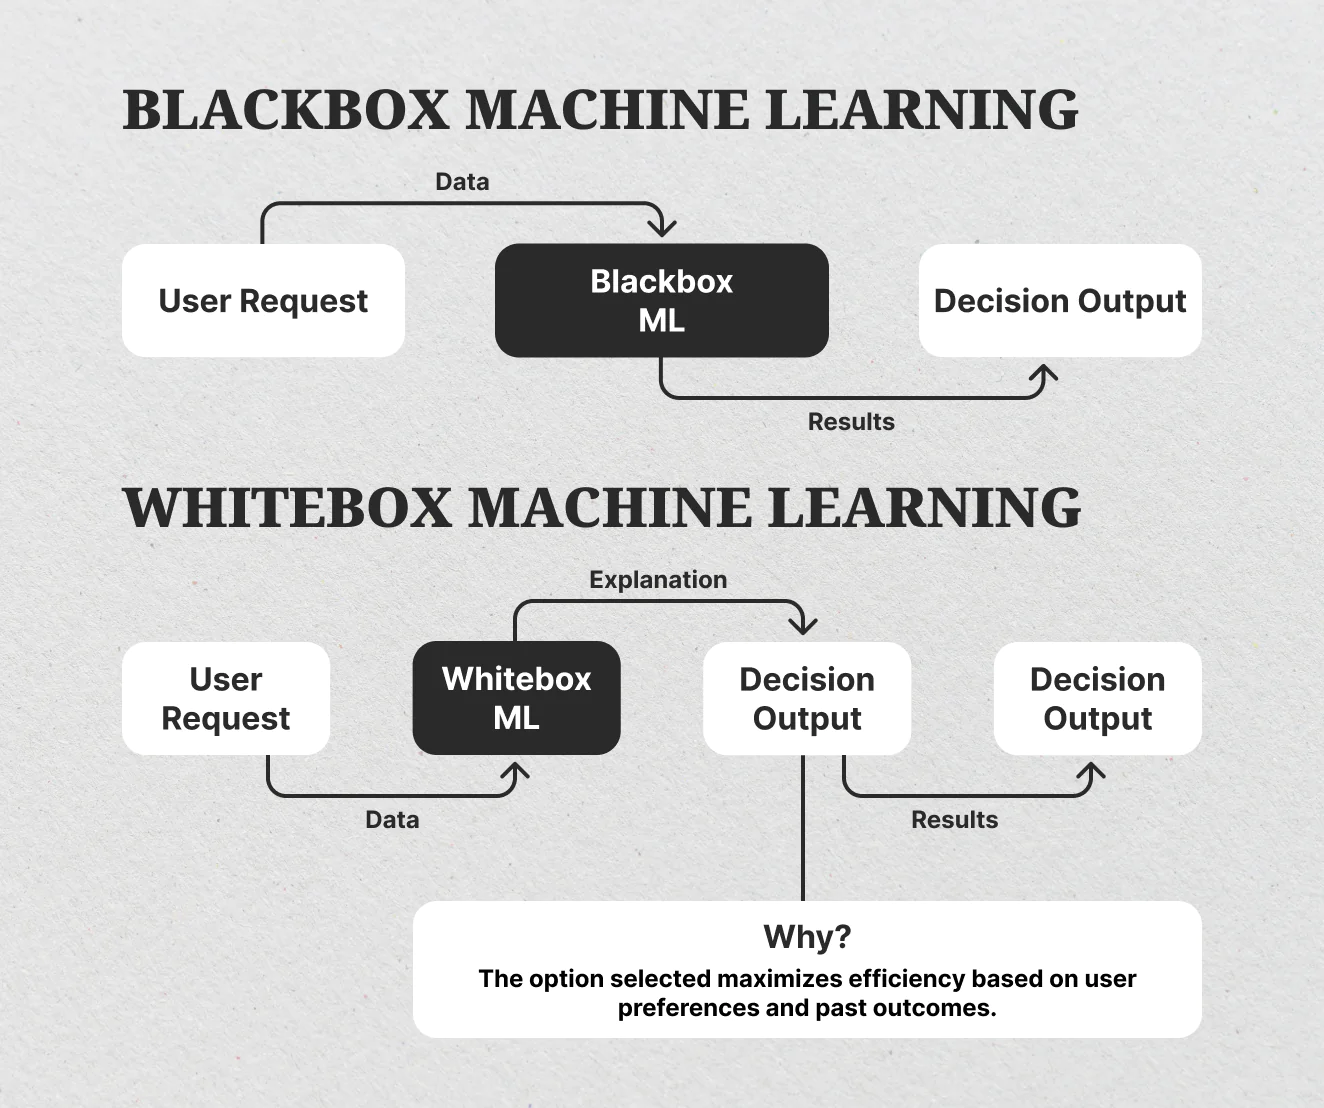
\includegraphics[width=0.8\textwidth]{My-Thesis/Chap1/images/taxonomy.png}
    \caption{Taxonomie des méthodes d'explicabilité : boîte noire (indépendante du modèle), et boîte blanche (modèle interprétable). L'axe vertical représente le niveau d'interprétabilité}
    \label{fig:taxonomie_xai}
\end{figure}

\begin{itemize}
    \item \textbf{Approches indépendantes du modèle (boîte noire)} : Ces méthodes analysent les entrées et sorties du modèle sans accéder à sa structure interne. Elles sont flexibles, car applicables à tout type de modèle, mais reposent souvent sur des corrélations plutôt que sur des causalités. Par exemple, des outils comme LIME ou SHAP quantifient l'impact des variables d'entrée sur les prédictions \cite{guidotti2018}. Elles sont particulièrement adaptées lorsque la priorité est de fournir des explications rapides et générales, sans nécessiter une expertise approfondie de l'architecture sous-jacente. Cependant, leur fidélité peut être limitée, car elles ne capturent pas toujours les mécanismes précis du modèle.
    % \begin{figure}
    %     \centering
    %     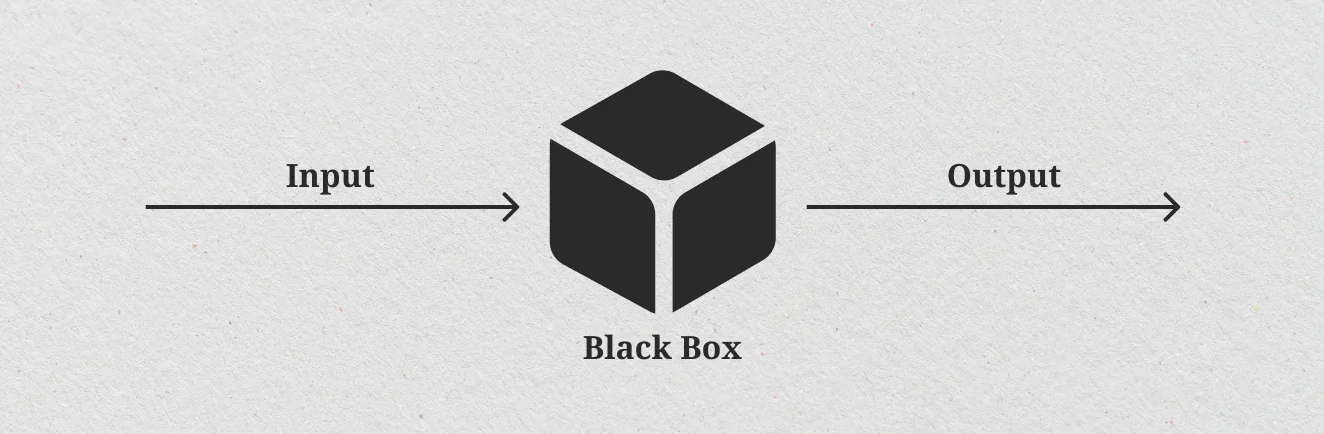
\includegraphics[width=0.6\linewidth]{chap1//images/blackbox_ai.png}
    %     \caption{modele boite noire}
    %     \label{fig:enter-label}
    % \end{figure}

    \item \textbf{Approches dépendantes du modèle (boîte grise)} : Ces techniques exploitent les paramètres internes du modèle, comme les poids des neurones ou les activations des couches, pour générer des explications. Elles offrent une meilleure fidélité, car elles reflètent directement le fonctionnement du modèle, mais sont contraintes par l'architecture spécifique (par exemple, CNN ou LSTM) \cite{jouis2020}. Des méthodes comme Grad-CAM, qui produit des cartes de chaleur pour les réseaux convolutifs, permettent de visualiser les régions influentes d’une entrée \cite{selvaraju2017gradcam}. Ces approches conviennent aux scénarios où une compréhension fine du modèle est nécessaire, mais elles exigent des compétences techniques pour interpréter les résultats.

    \item \textbf{Modèles interprétables (boîte blanche)} : Ces approches intègrent l'explicabilité dès la conception du modèle, en utilisant des architectures intrinsèquement transparentes, comme les mécanismes d'attention ou des réseaux simplifiés \cite{jouis2020}. Elles garantissent une compréhensibilité élevée, car les explications sont directement dérivées des paramètres du modèle, mais peuvent sacrifier une partie des performances par rapport aux modèles complexes. Elles sont idéales pour les applications où la transparence est une priorité absolue, comme dans les systèmes critiques soumis à des réglementations strictes.

\end{itemize}

Chaque catégorie présente des avantages et des limites, qui dépendent des contraintes du projet et des attentes des utilisateurs. Par exemple, dans le cadre du contrôle d'accès, les approches indépendantes du modèle peuvent être privilégiées pour leur flexibilité, tandis que les modèles interprétables sont mieux adaptés pour répondre aux exigences légales de transparence, comme celles imposées par le RGPD \cite{guidotti2018}. Le choix d’une méthode doit donc équilibrer la fidélité des explications, leur compréhensibilité et les ressources disponibles pour leur mise en œuvre.





\mySubSection{Méthodes Spécifiques d’Explicabilité}{}

Cette section détaille les principales méthodes d'explicabilité utilisées pour rendre les modèles d'apprentissage profond plus transparents, en se concentrant sur leur application potentielle au contrôle d'accès. Ces approches sont classées en trois catégories selon leur dépendance à l'architecture du modèle : approches indépendantes du modèle, approches dépendantes du modèle, et modèles interprétables. Chaque méthode est illustrée, lorsque pertinent, par des visualisations issues de la littérature.

\mySubSubSection{Approches indépendantes du modèle}{}

Les approches indépendantes du modèle, souvent qualifiées d'agnostiques, permettent d'expliquer les prédictions sans nécessiter une connaissance approfondie de la structure interne du modèle. Elles se basent principalement sur l'analyse des relations entre les entrées et les sorties, offrant ainsi une grande flexibilité d'application.

\paragraph{LIME (Local Interpretable Model-agnostic Explanations)}  
L'outil LIME, proposé par \cite{ribeiro2016lime}, génère des explications locales en approximant le comportement d'un modèle complexe autour d'une instance spécifique à l'aide d'un modèle linéaire simple. Pour une prédiction donnée, LIME identifie les variables d'entrée ayant le plus d'impact, comme les mots dans un texte ou les pixels dans une image, et quantifie leur influence positive ou négative sur la décision. Cette méthode est particulièrement utile pour expliquer des décisions dans des contextes comme le contrôle d'accès, où il peut être nécessaire de justifier pourquoi un accès a été refusé en mettant en évidence des facteurs clés (par exemple, une tentative d'accès à une heure inhabituelle).  

\begin{figure}[h]
    \centering
    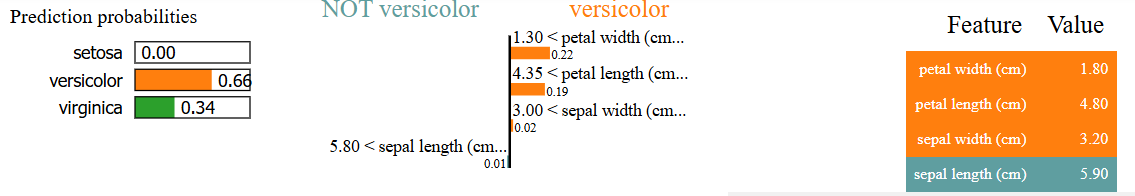
\includegraphics[width=0.8\textwidth]{My-Thesis/Chap1/images/lime_explanation.png}
    \caption{LIME : Visualisation de l’importance des mots dans une prédiction textuelle, où chaque mot est associé à un poids reflétant son influence sur la classe prédite \citep{ribeiro2016why}.}
    \label{fig:lime}
\end{figure}

\paragraph{Ancres}  
Les Ancres, une amélioration de LIME proposée par \citet{ribeiro2018anchors}, fournissent des explications sous forme de règles logiques définissant le contexte dans lequel une prédiction est valide. Par exemple, pour une décision de contrôle d'accès, une ancre pourrait être : "Si l’utilisateur tente d’accéder depuis un emplacement non autorisé et à une heure inhabituelle, alors l’accès est refusé." Ces règles sont construites pour maximiser la précision (fidélité au modèle) et la couverture (généralisation à d’autres instances similaires). Cette approche est particulièrement adaptée pour des systèmes nécessitant des justifications claires et compréhensibles par des utilisateurs non techniques.

\begin{figure}[h]
    \centering
    \includegraphics[width=0.8\textwidth]{My-Thesis/Chap1/images/anchor_explanation.png}
    \caption{Anchor : Visualisation des parties importantes d’une entrée (par exemple, mots ou régions d’image) définissant une règle d’explication pour une prédiction spécifique \citep{ribeiro2018anchors}.}
    \label{fig:anchor}
\end{figure}

\paragraph{Valeurs de Shapley et SHAP}  
Inspirées de la théorie des jeux, les valeurs de Shapley quantifient la contribution de chaque variable d’entrée à une prédiction \citep{lundberg2017shap}. Le module SHAP (\textit{Shapley Additive Explanations}) optimise ce calcul pour le rendre applicable à des modèles complexes, en fournissant une mesure de l’importance des variables sous forme de scores additifs. Par exemple, dans le cadre du contrôle d’accès, SHAP pourrait révéler qu’une tentative d’accès a été refusée principalement en raison de l’historique des connexions de l’utilisateur. Cependant, cette méthode peut être difficile à interpréter pour des utilisateurs non experts en raison de la complexité des calculs et de la nécessité d’un post-traitement pour simplifier les résultats.

\paragraph{Limites}  
Les approches indépendantes du modèle, bien que flexibles, présentent des limites. Elles mettent en évidence des corrélations entre entrées et sorties, mais ne garantissent pas une compréhension causale des décisions. De plus, leur complexité peut rendre les explications difficiles à assimiler pour des utilisateurs sans expertise technique, en particulier dans des domaines comme le contrôle d’accès où les explications doivent être conformes aux réglementations.

\mySubSubSection{Approches dépendantes du modèle}{}

Les approches dépendantes du modèle exploitent la structure interne du modèle pour générer des explications plus fidèles à son fonctionnement. Elles nécessitent une connaissance de l’architecture, ce qui limite leur applicabilité mais améliore leur précision.

\paragraph{Grad-CAM}  
La méthode Grad-CAM (\textit{Gradient-weighted Class Activation Mapping}), proposée par \cite{selvaraju2017gradcam}, génère des cartes de chaleur pour visualiser les régions d’une entrée (généralement une image) influençant une prédiction dans un réseau convolutif (CNN). Bien que principalement utilisée pour l’analyse d’images, cette méthode pourrait être adaptée au contrôle d’accès pour des données visuelles, comme des captures d’écran de tentatives d’accès frauduleuses, en mettant en évidence les zones critiques de l’image. La fidélité de Grad-CAM à la décision du modèle en fait un outil puissant, mais son application est restreinte aux architectures convolutives.


\begin{figure}[h]
    \centering
    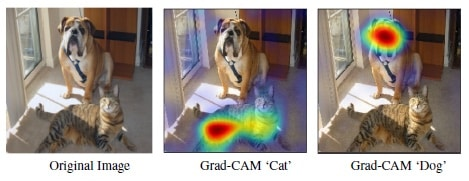
\includegraphics[width=0.8\textwidth]{My-Thesis/Chap1/images/gradcam_visualization.png}
    \caption{Visualisation d'une explication Grad-CAM.}
    \label{fig:gradcam}
\end{figure}

dans la figure \ref{fig:gradcam}, la Carte de chaleur met en évidence les régions d’une image influençant la classification dans un réseau convolutif, comme les zones pertinentes pour identifier une classe spécifique, l'un pour les chiens et l'autre pour les chats. \citep{GradCAMImage}

\paragraph{Analyse des LSTM}  
Les réseaux Long Short-Term Memory (LSTM) sont largement utilisés pour l’analyse de séquences, comme les logs d’accès dans un système de contrôle. \citet{karpathy2015visualizing} proposent d’étudier les activations des cellules LSTM pour comprendre les motifs détectés, comme la reconnaissance de motifs spécifiques dans un texte (par exemple, des guillemets indiquant une citation). Dans le contexte du contrôle d’accès, cette méthode pourrait révéler pourquoi un modèle a identifié une séquence d’actions comme suspecte. Cependant, l’analyse des activations est complexe et nécessite une exploration approfondie, ce qui peut limiter son accessibilité.


\begin{figure}[h]
    \centering
    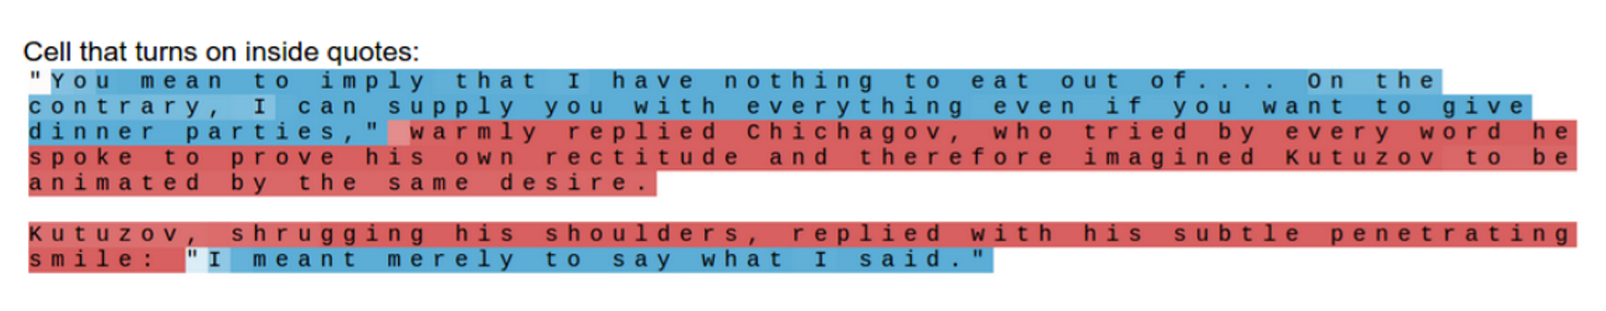
\includegraphics[width=0.8\textwidth]{My-Thesis/Chap1/images/lstm_activation.png}
    \caption{Activation d’une cellule en fonction des guillemets dans le texte : Visualisation des activations d’une cellule LSTM détectant des motifs textuels spécifiques, comme les guillemets \citep{karpathy2015visualizing}.}
    \label{fig:lstm}
\end{figure}

\paragraph{Avantages et inconvénients}  
Les approches dépendantes du modèle offrent une grande fidélité, car elles s’appuient directement sur les mécanismes internes du modèle. Elles sont particulièrement utiles pour des experts souhaitant auditer un système de contrôle d’accès. Cependant, leur dépendance à l’architecture limite leur généralisation, et leur complexité peut poser des défis pour des explications destinées à des utilisateurs non techniques.

\mySubSubSection{Modèles interprétables}{}

Les modèles interprétables, ou boîtes blanches, sont conçus pour être transparents par leur architecture, réduisant ainsi le besoin d’analyses post-entraînement.

\paragraph{Mécanismes d’attention}  
Les mécanismes d’attention, décrits par \cite{lin2017structured}, permettent de visualiser les poids attribués aux différentes parties d’une entrée, comme les mots dans une phrase. Dans une tâche de traduction, par exemple, les poids d’attention mettent en évidence les correspondances entre mots source et cible. Appliqués au contrôle d’accès, ces mécanismes pourraient identifier les éléments clés d’une requête d’accès (par exemple, un identifiant utilisateur ou une adresse IP) influençant la décision. Cette approche est intuitive et ne nécessite pas de calculs supplémentaires après l’entraînement, mais elle est spécifique aux modèles intégrant une couche d’attention.



\begin{figure}[h]
    \centering
    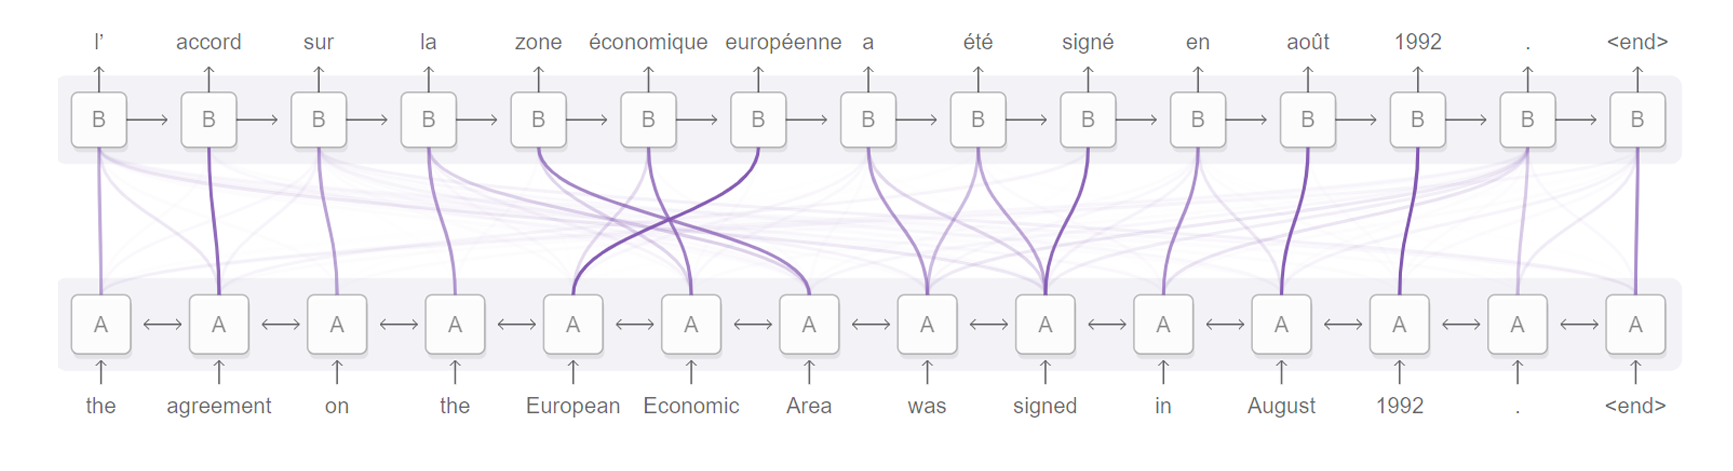
\includegraphics[width=0.8\textwidth]{My-Thesis/Chap1/images/attention_visualization.png}
    \caption{Visualisation de l’attention pour une tâche de traduction : Représentation des poids d’attention montrant les correspondances entre les mots d’une phrase source et sa traduction \cite{lin2017structured}.}
    \label{fig:attention}
\end{figure}

\paragraph{Architectures simplifiées}  
Les architectures simplifiées, comme celles étudiées par \citet{hasani2019compact}, utilisent des réseaux compacts avec un faible nombre de neurones pour faciliter l’analyse des activations. Par exemple, un réseau inspiré du système nerveux d’un ver peut accomplir des tâches complexes tout en restant interprétable grâce à sa simplicité. Dans le contrôle d’accès, de telles architectures pourraient être utilisées pour des décisions simples, comme l’authentification de base, mais elles risquent de manquer de puissance pour des scénarios complexes impliquant de grandes quantités de données.

\paragraph{Avantages et limites}  
Les modèles interprétables offrent une transparence native, idéale pour des applications nécessitant des explications immédiates et compréhensibles. Cependant, leur simplicité peut entraîner une perte de performance par rapport aux modèles plus complexes, ce qui pose un défi dans des contextes comme le contrôle d’accès où la précision est critique.





\mySubSection{Évaluation de l’Explicabilité}{}
L’évaluation de l’explicabilité des modèles d’intelligence artificielle, en particulier des modèles d’apprentissage profond, représente un défi majeur en raison de l’absence de métriques universellement acceptées \cite{jouis2020}. Contrairement aux métriques de performance classiques, telles que la précision ou le rappel, qui sont bien établies, l’explicabilité nécessite des mesures qui tiennent compte à la fois de la fidélité des explications au modèle et de leur compréhensibilité pour les utilisateurs. Cette difficulté est exacerbée par la diversité des contextes d’application et des publics cibles, qui vont des experts techniques aux utilisateurs non initiés.

Les approches pour évaluer l’explicabilité se divisent généralement en deux catégories : les métriques objectives et les métriques subjectives. Les métriques objectives incluent des indicateurs tels que la précision des explications (c’est-à-dire leur capacité à refléter fidèlement les décisions du modèle), le temps de réponse des utilisateurs lorsqu’ils doivent interpréter une explication, ou encore leur capacité à prédire les sorties du modèle à partir des explications fournies \cite{ribeiro2016lime}. Par exemple, dans le cadre de l’évaluation de la méthode des Ancres, des tests avec utilisateurs réels ont montré que des explications sous forme de règles permettent une meilleure compréhension des décisions par rapport à des explications basées sur des poids \cite{ribeiro2016lime}. Les métriques subjectives, quant à elles, se concentrent sur l’acceptabilité des explications et la confiance qu’elles inspirent aux utilisateurs. Ces métriques sont souvent recueillies via des enquêtes ou des retours qualitatifs, mettant en lumière l’importance de la simplicité et de la clarté des explications.


Un aspect crucial de l’évaluation réside dans la prise en compte du contexte et des besoins spécifiques des utilisateurs \cite{dam2018}. Une explication efficace doit être adaptée au niveau d’expertise de son destinataire, qu’il s’agisse d’un administrateur système analysant une décision de contrôle d’accès ou d’un utilisateur final cherchant à comprendre une restriction d’accès. Par exemple, une visualisation comme celle de LIME (voir Figure~\ref{fig:lime}) peut être intuitive pour un utilisateur technique, mais nécessitera une simplification pour un public non expert. De plus, l’évaluation doit refléter l’environnement fonctionnel réel du modèle, afin de garantir que les explications sont pertinentes et utiles dans des scénarios concrets.

\mySubSection{Relevance pour le Contrôle d’Accès}{}
L’application des méthodes d’explicabilité au domaine du contrôle d’accès répond à des besoins critiques en matière de transparence, de conformité réglementaire et de confiance des parties prenantes. Dans des systèmes où les décisions d’accès aux données ou aux traitements sont automatisées, comme dans les infrastructures cloud ou les systèmes IoT, les modèles d’apprentissage profond offrent une grande adaptabilité, mais leur opacité peut compromettre leur adoption. Les réglementations telles que le Règlement Général sur la Protection des Données (RGPD), en particulier son article 22, exigent que les décisions automatisées soient accompagnées d’explications compréhensibles \cite{desmoulin2019}. Cette exigence légale souligne l’importance de méthodes XAI capables de produire des justifications claires et conformes.

Des outils comme LIME ou les Ancres offrent des solutions prometteuses pour le contrôle d’accès. Par exemple, LIME peut être utilisé pour expliquer une décision de refus d’accès en mettant en évidence les facteurs clés, tels que des anomalies dans les métadonnées de connexion (adresse IP, heure d’accès, etc.). Une visualisation comme celle présentée dans la Figure~\ref{fig:lime} pourrait montrer l’importance relative de chaque attribut dans la décision, facilitant ainsi l’audit par un administrateur. De même, les Ancres peuvent générer des règles explicites, comme « Si l’utilisateur se connecte depuis une localisation non autorisée ET à une heure inhabituelle, alors l’accès est refusé », offrant une justification intuitive et vérifiable pour une règle d’accès dynamique \cite{ribeiro2016lime}.

% \begin{figure}[h]
%     \centering
%     \includegraphics[width=0.8\textwidth]{chap1/images/anchor_explanation.png}
%     \caption{Représentation d’une explication avec la méthode des Ancres.}
%     \label{fig:anchor}
% \end{figure}

Cependant, l’intégration de l’explicabilité dans les systèmes de contrôle d’accès soulève des défis spécifiques. Tout d’abord, il est nécessaire de trouver un équilibre entre la performance des modèles, qui repose souvent sur des architectures complexes, et leur explicabilité, qui favorise des explications simples et directes. Ensuite, les explications doivent répondre aux contraintes légales tout en restant accessibles à des utilisateurs variés, allant des régulateurs aux employés \cite{desmoulin2019}. Enfin, les biais potentiels dans les données d’entraînement, qui pourraient conduire à des décisions discriminatoires (par exemple, un refus d’accès basé sur des corrélations démographiques), doivent être détectés et corrigés grâce à des outils d’explicabilité comme SHAP ou LIME.

\mySubSection{Conclusion de la Section}{}
Cette section a exploré les concepts fondamentaux de l’\textit{Explainable Artificial Intelligence} (XAI), en mettant l’accent sur les méthodes d’explicabilité, leur évaluation, et leur application au contrôle d’accès. Les approches comme LIME, les Ancres, et les mécanismes d’attention offrent des moyens concrets pour surmonter l’opacité des modèles d’apprentissage profond, tandis que l’évaluation de l’explicabilité nécessite une combinaison de métriques objectives et subjectives adaptées au contexte. Dans le domaine du contrôle d’accès, l’XAI joue un rôle clé pour garantir la transparence, la conformité aux réglementations, et la confiance des utilisateurs, tout en posant des défis liés à l’équilibre entre performance et compréhensibilité.

L’analyse de ces concepts prépare le terrain pour les sections suivantes du chapitre, qui examineront en détail les systèmes de contrôle d’accès traditionnels et basés sur l’IA, ainsi que les limites des approches existantes en matière d’explicabilité. Ces discussions permettront de mieux contextualiser la nécessité d’une approche XAI spécifiquement adaptée aux besoins du contrôle d’accès.
